\documentclass[10pt,a4paper]{article}
\usepackage[latin1]{inputenc}
\usepackage{amsmath}
\usepackage{amsfonts}
\usepackage{amssymb}
\usepackage{graphicx}
\usepackage[obeyspaces]{url}
\usepackage[colorlinks,urlcolor=blue]{hyperref}

\title{Windows installation guide for Tosca 2016}
\date{} % blank date

\begin{document}
	\maketitle
	
	\section*{Compatibility with Abaqus}
	Tosca 2016 is compatible with Abaqus 2016. It will not work with Abaqus 6.14 and below.
	
	\section{Licence Requirements}
	Before installing Tosca please read the \href{https://www.applications.itservices.manchester.ac.uk/show_product.php?id=184&tab=licensing}{licence requirements}, in particular noting:
	
	Only appropriately authorised support staff may make physical copies of the software or documentation.
	Tosca may only be installed on computers owned by the University of Manchester; it may not be installed on computers owned by staff or students.
	With limited exceptions use of Tosca by students is limited to on-campus facilities.
	Tosca on-line documentation may not be made available over the open internet.
	
	\section{Installation}
	\subsection{Documentation}
	Uses the same installer as Isight, so if you the Isight documentation has already been installed, you can skip this step.
	
	Mount \path{Isight_Tosca_2016_documentation.iso} and run \path{\1\setup.exe}
	
	\subsection{Software}
	\begin{itemize}
		\item Mount \path{Tosca_2016_Win_Lin.iso} then run \path{\1\setup.exe}
		\item Select which interfaces you want to set up. e.g. Specify Abaqus solver executable location (default locations shown in screenshots below).
		
		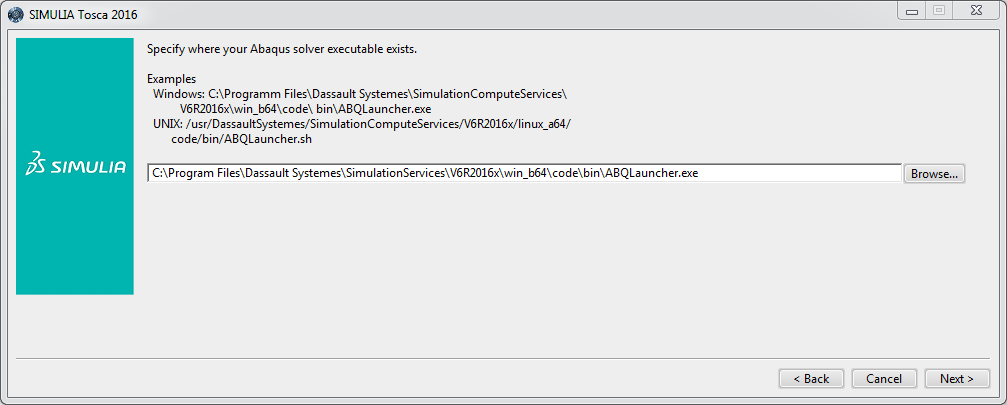
\includegraphics[width=0.9\textwidth]{tosca2016_abaqus_solver_location}
		
		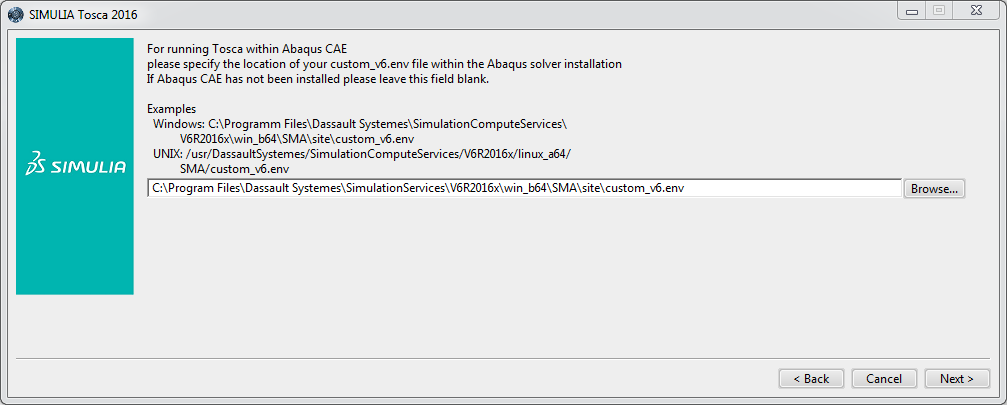
\includegraphics[width=0.9\textwidth]{tosca2016_abaqusCAE_location}
		
		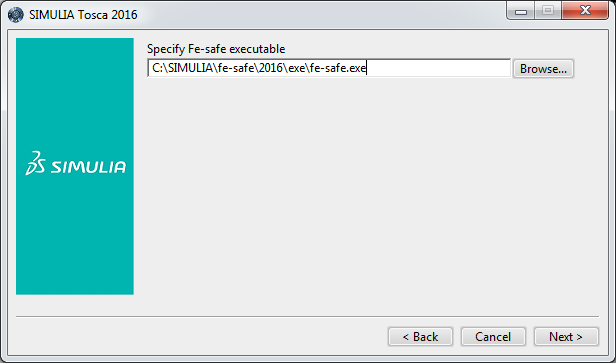
\includegraphics[width=0.9\textwidth]{tosca2016_fesafe_setup_guess}
		
		\item The type of licence server is \textbf{Flexnet} and the server addresses are shown below
		
		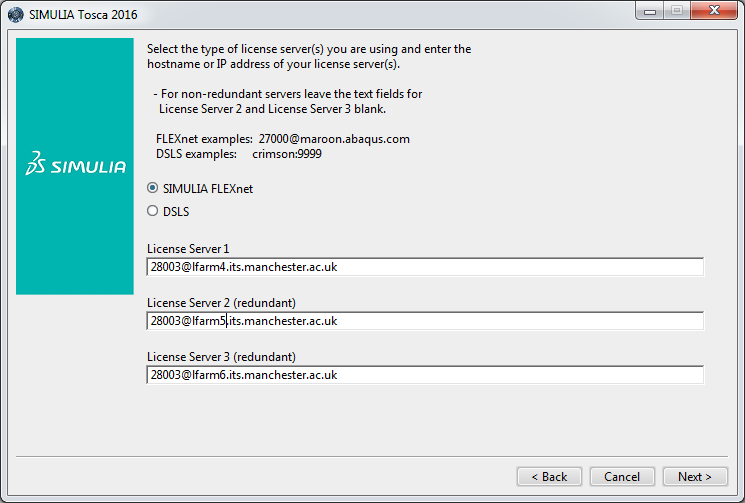
\includegraphics[width=0.9\textwidth]{tosca2016_licence}
		
		\break
		
		\item Documentation 
		
		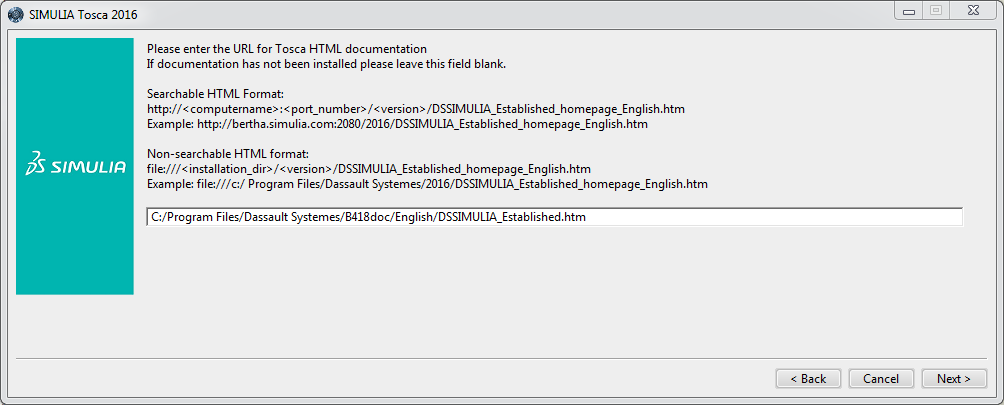
\includegraphics[width=0.9\textwidth]{tosca2016_nonsearchable_documentation}
	\end{itemize}
	
	\section{Post-installation tasks}
	In order to get documentation working, some modification are required to the following file: \path{[Tosca_install_path]\win_b64\code\command\ToscaStructureGui.bat} - if you accepted the defaults then this will be \path{C:\SIMULIA\Tosca\2016\win_b64\code\command\ToscaStructureGui.bat} 
	
	The final line (line 18) should be replaced with the following: 
	
	\smallskip
	\noindent
	\path{"%tosca%\code\jre\currentjre\bin\java.exe" "-Dtosca.browser=C:\Program Files\Internet Explorer\iexplore.exe" "-Dtosca.home=%tosca%" "-Dtosca.docroot=file:///C:/Program Files/Dassault Systemes/B418doc/English/DSSIMULIA_Established.htm" -classpath "%tosca%\docs\java\SMATsoMathPlot.jar;%tosca%\docs\java\SMATsoClassicGui.jar" toscagui.TOSCAgui}
	
	\smallskip
	Note that copying and pasting will probably introduce line breaks - this should be all one line, so you need to remove any line breaks.
	
	You don't have to set IE as your browser, however be warned that the documentation doesn't work with Chrome.
\end{document}	